\section*{Problem 2: Equal Ripple Filter}
\addcontentsline{toc}{section}{Problem 2: Equal Ripple Filter}

\subsection*{Ideal Band-Stop Filter}
\addcontentsline{toc}{subsection}{Ideal Band-Stop Filter}
The first thing to do is identify the component values based on the required
order (N = 3) and the type of filter (equal ripple or Chebysev). Doing so yields:

\begin{table}[H]
    \centering
    \caption{Lumped Component Values}
    \label{tab:3a_lumped_component_values}
    \begin{tabular}{|c|c|}
        \hline $\text{g}_{\text{i}} $ & Associated $\text{g}_{\text{value}} $ \\
        \hline $ g_1 $ & 1.5963 \\
        \hline $ g_2 $ & 1.0967 \\
        \hline $ g_3 $ & 1.5963 \\
        \hline $ g_4 $ & 1.0 \\
        \hline
    \end{tabular}
\end{table}

I will choose, again, a shunt capacitor as the leading element in my low-pass
filter prototype. In transforming from the low-pass filter prototype to the
band-stop design I will need to transform the inductors into tank LC circuits
and the capacitors into series LC circuits. The resistors will simply scale with
the impedance scaling. The relevant transformations are given below:

\[ 
    C \quad \rightarrow \quad L^s = \frac{1}{\Delta \cdot C} \quad,\quad C^s = \frac{\Delta
    \cdot C}{\omega_0^2}
\]

where the superscript ``s'' denotes a series LC element and $\Delta = \omega_2
- \omega_1$ (the stop-band bandwidth), $\omega_0 = \sqrt{\omega_1\omega_2}$ is
the geometric mean of the stop-band bandwidth. Similarly for the inductor
transformation we have:

\[ 
L \quad \rightarrow \quad C^t = \frac{1}{\Delta \cdot L} \quad,\quad L^t = \frac{\Delta
\cdot L}{\omega_0^2}
\]

where the same definitions as previously defined for the capacitor hold. In this
case, we know the fractional bandwidth is $10 \%$ and that the center frequency
(the midpoint of the two endpoints of the stop-band $\omega_1$ and $\omega_2$)
is \SI{3}{\giga\hertz}. Thus, we \textbf{could} construct the following two relationships:

\[
    \omega_{center} = \frac{\omega_1 + \omega_2}{2} \quad,\quad
    \text{BW}_{\text{frac}} = \frac{\omega_2 - \omega_1}{\omega_{center}}
\]

We have been given $\text{BW}_{\text{frac}}$ and $\omega_{center}$. This allows
us to solve for $\omega_1$, $\omega_2$ and $\omega_0$. However, the above
definition for the center frequency is not typically what is used. Instead, the
geometric mean of $\omega_1$ and $\omega_2$ (which is $\omega_0$) is what is
defined as the center frequency of the band-stop filter. Thus, $\omega_0 =
\SI{3}{\giga\hertz}$. So, we actually have the following two equations:

\[ 
    \omega_{center} = \omega_0 = \sqrt{\omega_1 \omega_2} \quad,\quad
    \text{BW}_{\text{frac}} = \frac{\Delta}{\omega_0} = \frac{\omega_2 -
    \omega_1}{\omega_0}
\]

Solving the above equations for $\omega_1$ and $ \omega_2 $ yields:

\[ 
    \omega_1 \approx \SI{2.85}{\giga\hertz} \quad,\quad \omega_2 \approx
    \SI{3.15}{\giga\hertz} 
\]

Now, in the chosen topology, $g_1, g_3$ represent capacitors and $g_2$
represents an inductor. I will start by transforming the capacitors. First,
though, I will obtain the capacitance and inductance after impedance scaling.
The reference impedance for this problem is \SI{75}{\ohm}. Thus, the capacitor
and inductor values are as shown in \ref{tab:2_comp_values}

\begin{table}[H]
    \centering
    \caption{Component Values after Impedance Scaling}
    \label{tab:2_comp_values}
    \begin{tabular}{|c|c|}
    \hline $ C_1 = C_3$ & \SI{21.2}{\milli\farad} \\
    \hline $ L_2 $ & \SI{82.3}{\henry} \\
    \hline
    \end{tabular}
\end{table}

The series elements are calculated from the capacitor value and are given as in
\ref{tab:2_series_elements}.

\begin{table}[H]
    \centering
    \caption{Series LC elements after Band-Stop Transformation}
    \label{tab:2_series_elements}
    \begin{tabular}{|c|c|}
        \hline L & \SI{25.0}{\nano\henry} \\
        \hline C & \SI{112}{\femto\farad} \\
        \hline
    \end{tabular}
\end{table}

Doing the same thing for the inductor transformation we see in
\ref{tab:2_tank_elements}:

\begin{table}[H]
    \centering
    \caption{Tank LC Elements after Band-Stop Transformation}
    \label{tab:2_tank_elements}
    \begin{tabular}{|c|c|}
    \hline L & \SI{437}{\pico\henry} \\
    \hline C & \SI{6.45}{\pico\farad} \\
    \hline
    \end{tabular}
\end{table}

This leads to the design shown in the schematic in figures
\ref{fig:img/Problem2/IdealSchematic.PNG} and
\ref{fig:img/Problem2/IdealResults.PNG}.

\begin{figure}[H]
    \centering
    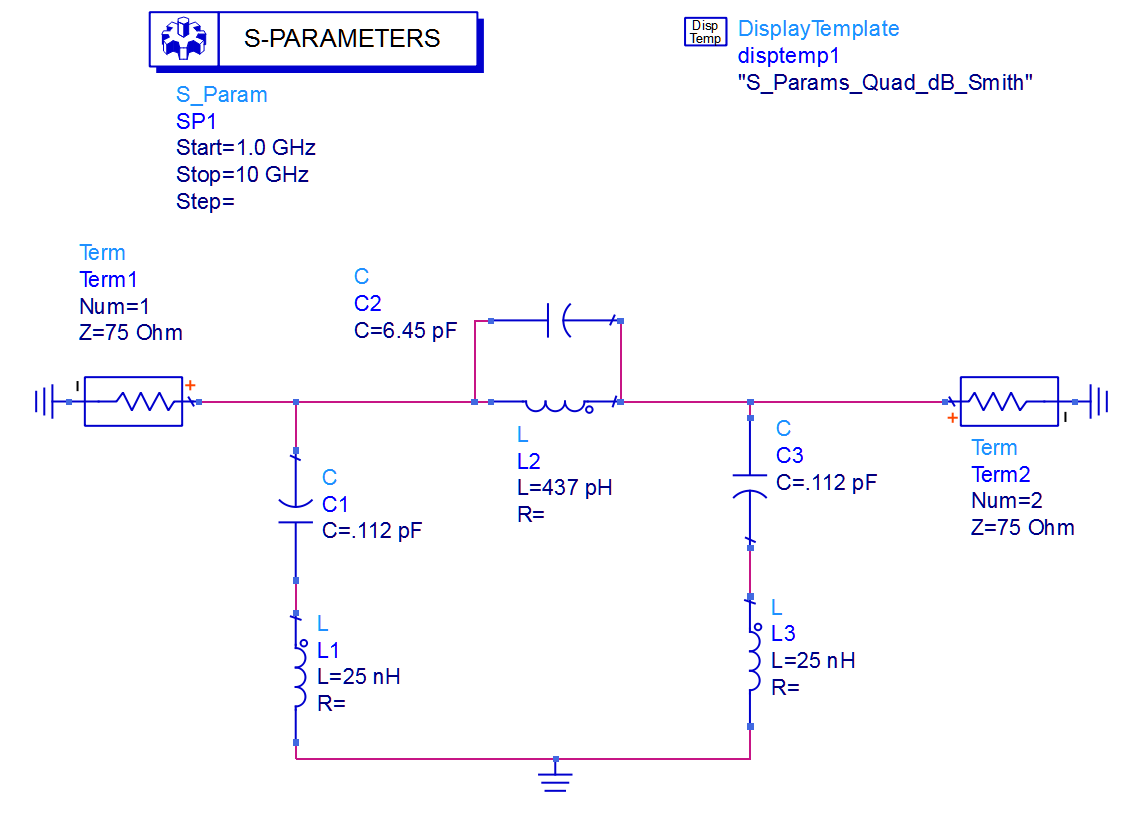
\includegraphics[width=0.8\linewidth]{img/Problem2/IdealSchematic.PNG}
    \caption{Schematic of the Ideal, Lumped-Element Band-Stop Filter}
    \label{fig:img/Problem2/IdealSchematic.PNG}
\end{figure}

\begin{figure}[H]
    \centering
    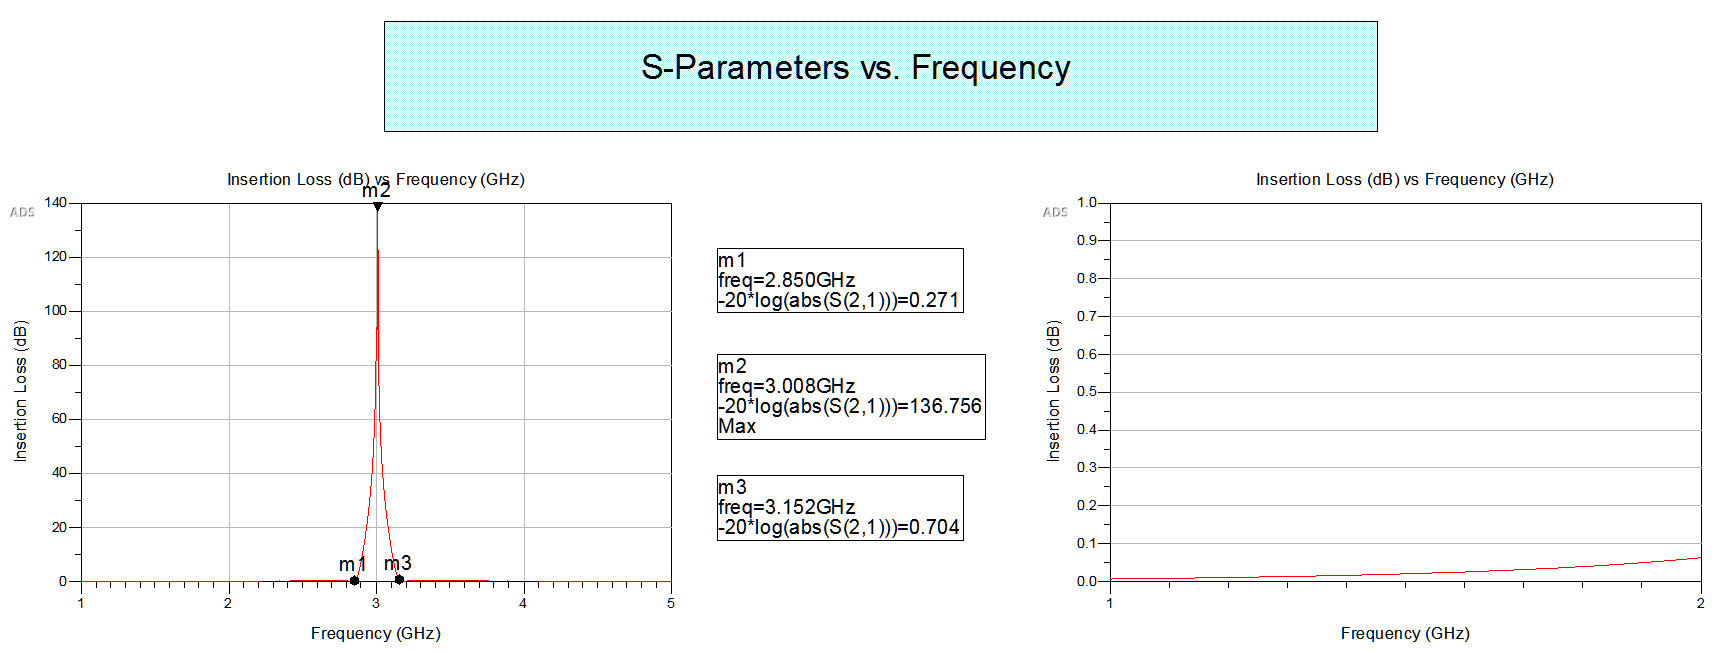
\includegraphics[width=0.8\linewidth]{img/Problem2/IdealResults.PNG}
    \caption{Results of Simulating the Ideal, Lumped-Element Band-Stop Filter}
    \label{fig:img/Problem2/IdealResults.PNG}
\end{figure}

I find it problematic that the passband shows no ripple and no insertion loss
even close to \SI{.5}{\deci\bel} but I have checked and re-checked my design. I
also checked my values against an online tool. They are consistent. Any feedback
would be greatly appreciated.

\subsection*{Lossy Band-Stop Filter}
\addcontentsline{toc}{subsection}{Lossy Band-Stop Filter}

Problem 1c: 1a and 1b with Steps and T-Junctions
Now, I just need to make the elements lossy. The capacitors are to have a
quality factor of 40 and the inductors are to have a quality factor of 20.
Assuming a series-lossy model for the inductor and a shunt-lossy model for the
capacitor we have the following relationships between Q, R, and the element
values:

\[ 
    R^L_s = \frac{X^L_s}{Q^L_s} \quad,\quad R^C_p = X^C_p Q^C_p
\]

where the superscript denotes the element type and the subscript denotes
whether the resistor is in parallel (p) or in series (s) with the inductor (L)
or capacitor (C). We can now solve for the four resistances for the four
elements:

\begin{table}[H]
    \centering
    \caption{Resistance of Each of the Imperfect Lumped Elements}
    \label{tab:lumped_element_resistance}
    \begin{tabular}{|c|c|}
        \hline $R_L$~\text{(series LC)} & $\frac{\omega_c L}{Q_L} \approx
        \SI{23.6}{\ohm}$ \\
        \hline $R_C$~\text{(series LC)} & $ \frac{Q_C}{\omega_c C}\approx
        \SI{18.9}{\kilo\ohm} $ \\
        \hline $R_L$~\text{(tank LC)} & $\frac{\omega_c L}{Q_L} \approx
        \SI{412}{\milli\ohm}$ \\
        \hline $R_C$~\text{(tank LC)} & $ \frac{Q_C}{\omega_c C}\approx
        \SI{329}{\ohm} $ \\
        \hline
    \end{tabular}
\end{table}

Inserting the above resistances into the design and simulating yields a much
lower attenuation over the stop-band. The bandwidth doesn't change significantly,
which is surprising since the peak flattens a lot. But, the \SI{3}{\deci\bel}
points are at almost the exact same frequencies. The results are given below in
figures \ref{fig:img/Problem2/NonIdealSchematic} and
\ref{fig:img/Problem2/NonIdealResults}

\begin{figure}[H]
    \centering
    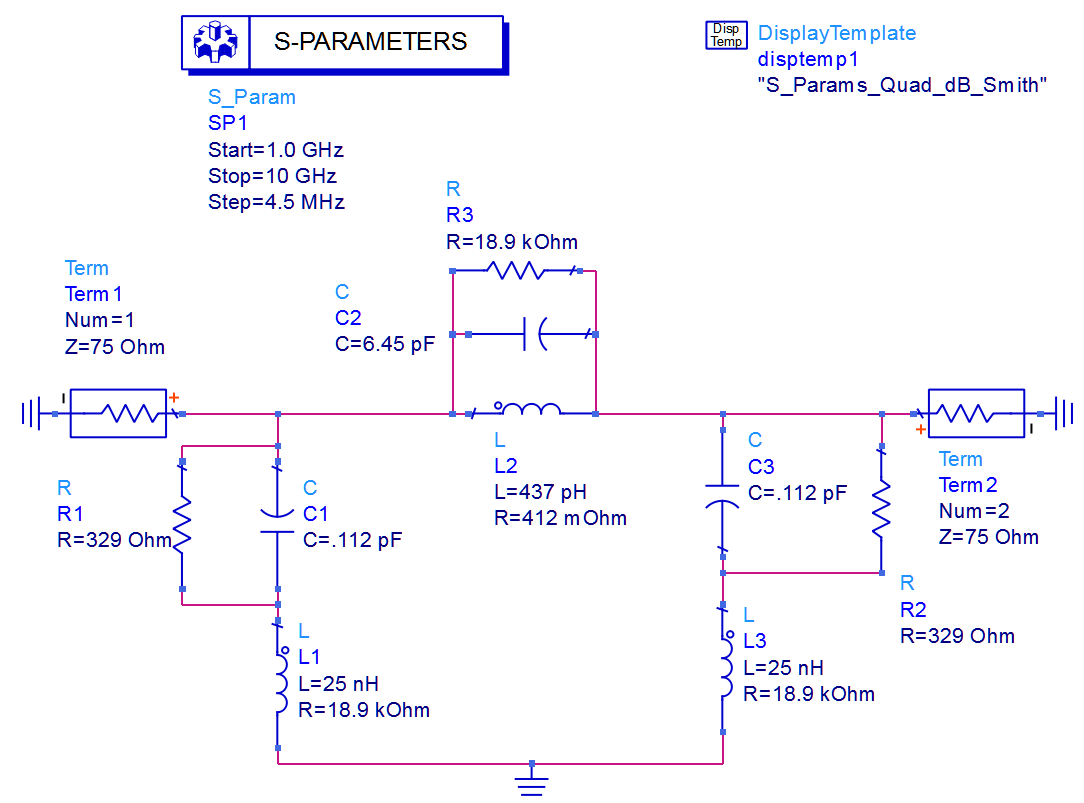
\includegraphics[width=0.8\linewidth]{img/Problem2/NonIdealSchematic.PNG}
    \caption{Schematic for the Non-Ideal Lumped-Element Band-Stop Filter}
    \label{fig:img/Problem2/NonIdealSchematic}
\end{figure}

\begin{figure}[H]
    \centering
    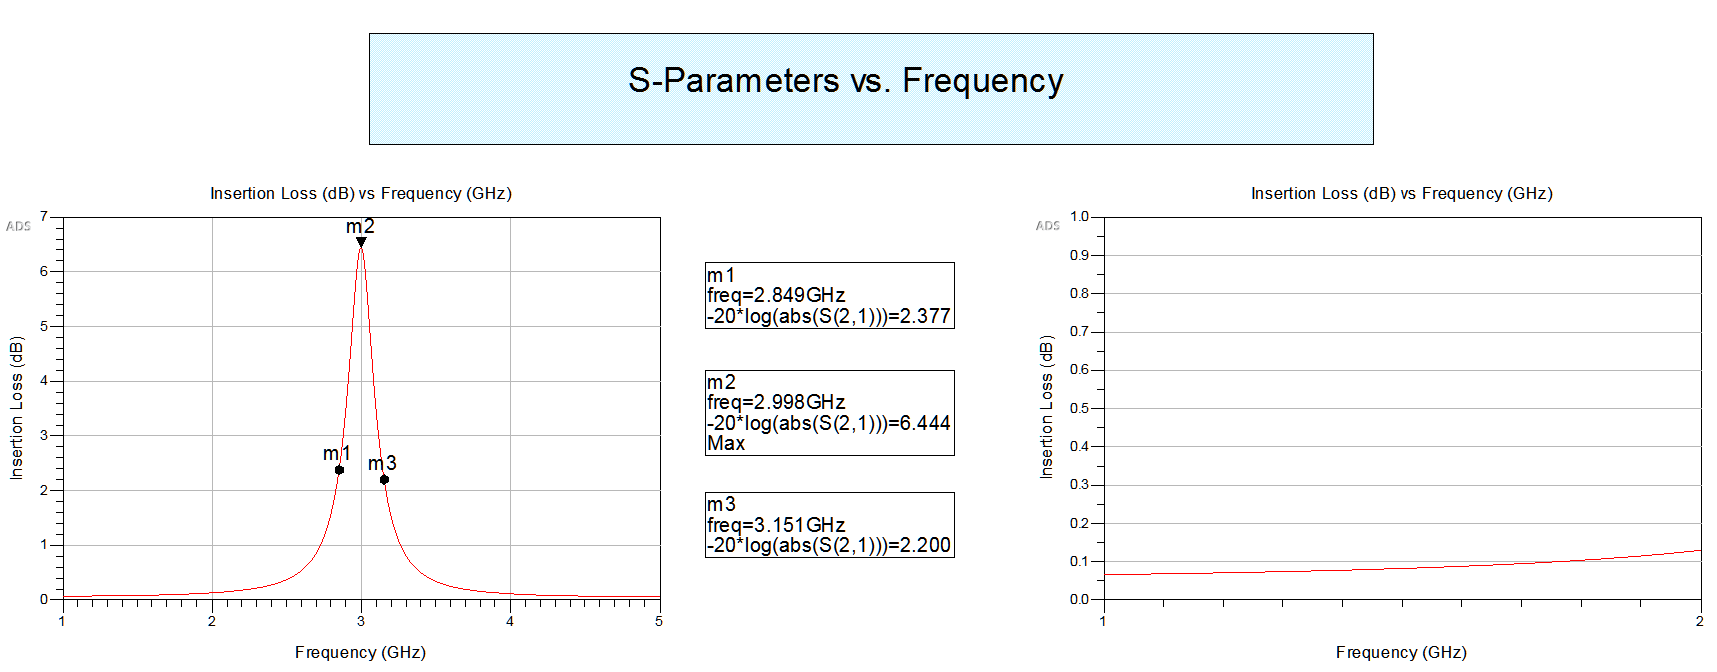
\includegraphics[width=0.8\linewidth]{img/Problem2/NonIdealResults.PNG}
    \caption{Results for the Non-Ideal Lumped-Element Band-Stop Filter}
    \label{fig:img/Problem2/NonIdealResults}
\end{figure}
